\documentclass[12pt]{article}
\usepackage{fullpage}
\usepackage{epsf}
\usepackage{amsmath}
\usepackage{amsthm}
\usepackage{txfonts,pxfonts,amsfonts}
\usepackage{epsfig}
\usepackage{caption}
\usepackage{subfig}
\usepackage{graphicx}
\usepackage[citecolor=blue,linkcolor=blue,colorlinks=true]{hyperref}
% \usepackage{algorithmic}
% \usepackage{algorithm}

\usepackage{booktabs} % For formal tables
\usepackage{xspace}
\usepackage{lipsum}
\usepackage{courier}
\usepackage{array,multirow}
\usepackage{float}

% \usepackage{hyperref}
\usepackage{listings}
\usepackage[ruled,linesnumbered]{algorithm2e}
\usepackage{url}

\lstset{
  escapeinside={\`}{\`}
}
\lstdefinestyle{rm}{mathescape,basicstyle=\normal\ttfamily}


\newcommand{\hlight}[1]{{\em #1}}
\newcommand{\REM}[1]{}
\newcommand{\name}{{\tt Falcon-Bi}\xspace}
\newcommand{\Graph}{\texttt{Graph}\xspace}
\newcommand{\GPU}{\texttt{GPU}\xspace}
\newcommand{\CPU}{\texttt{CPU}\xspace}
\newcommand{\Point}{\texttt{Point}\xspace}
\newcommand{\Edge}{\texttt{Edge}\xspace}


\def\reporttitle{Custom Code Generation for a Graph DSL}
\def\reportauthor{Bikash Gogoi}
\def\authorrollno{CS14B039}
\def\guide{Dr.~Rupesh Nasre (Dept of Computer Science \& Engineering, IIT Madras)}


\title{\reporttitle \\ {\small (Dual Degree Project - Interim Report)}}
\author{\reportauthor\ (\authorrollno)~\footnote{Guide : \guide}}
\date{\today}

\begin{document}
\maketitle

\begin{abstract}
We present challenges faced in making a domain-specific language (DSL) for graph algorithms adapt to varying requirements to generate a spectrum of efficient parallel codes. Graph algorithms are at the heart of several applications, and achieving high performance with them has become critical due to tremendous growth of irregular data. However, irregular algorithms are quite challenging to parallelize automatically, due to access patterns influenced by the input graph -- which is unavailable until execution. Former research has addressed this issue by designing DSLs for graph algorithms, which restrict generality, but allow efficient code-generation for various backends. Such DSLs are, however, too rigid, and do not adapt to changes in backends or to input graph properties or to both. We narrate our experiences in making an existing DSL, named Falcon, adaptive. The biggest challenge in the process is to not change the DSL code for specifying the algorithm. We illustrate the effectiveness of our proposal by auto-generating codes for vertex-based versus edge-based graph processing, synchronous versus asynchronous execution, and CPU versus GPU backends.
\end{abstract}

\tableofcontents

\section{Introduction} 
\subsection{Motivation}
Graphs model several real-world phenomena such as friendship, molecular interaction and co-authorship.
Several graph algorithms have been designed across domains to compute such relationships between entities.
Performance of these graph algorithms has become critical today due to explosive growth of unstructured data.
For instance, to simulate a simple physical phenomenon, an algorithm may have to work with billions of particles.

On the other side, computer hardware is witnessing rapid changes with new architectural innovations.
Exploiting these architectures demands complex coding and good compiler support.
The demand intensifies in the presence of parallelization.
It is not uncommon to see a twenty-line textbook graph algorithm implemented using several hundred lines of optimized parallel code.

It would be ideal if the algorithm is programmed at a high-level without worrying about the nuances of the hardware.
This gave rise to domain-specific languages (DSLs) for graph algorithms which allowed programmers to write complex algorithmic codes and took care of efficient parallel code generation~\cite{greenmarl, lighthouse, falcon}.
Such DSLs often disallow writing arbitrary programs, trading off generality for performance.
This makes programming parallel hardware easy, and adapting to changes manageable.

An example of a graph DSL is Falcon~\cite{falcon, dhfalcon} which supports a wide variety of backends: CPU, GPU, multi-GPU, heterogeneous processing, and distributed systems. 
It extends C language to allow graph processing being specified at a high-level.
Falcon provides special constructs (such as worklists and reductions) for simplifying algorithm specification and also aiding efficient code generation.
We choose Falcon because it supports a variety of backends.

Unfortunately, graph algorithms do not always have a fixed performance pattern.
The pattern varies depending upon the graph structure which is available only at runtime.
Such an \textit{irregular} pattern poses challenges in parallelizing graph algorithms and in optimizing them for efficient execution.
For instance, vertex-based processing works well for road networks, but social networks demand an edge-based processing.
Sequential processing of parallel loops demands synchronous execution, but independent loops can be more efficient with asynchronous processing.
Similarly, backend optimizations are quite different for different targets such as CPU and GPU.

Falcon (and other graph DSLs) allows writing code for a particular kind of processing. % UK- this is true for other DSLs, so ours is novel as such a dsl is lacking. needs to be highlighted.
The code written in Falcon DSL needs modifications for an alternative way of processing.
Various syntactic elements in the program need to be changed for the alternative way. 
Thus, code needs to be written separately for vertex-based and edge-based processing, for instance.
While this is a step better than being totally rigid, it would be helpful if one could generate different kind of code from the \textit{same DSL specification}.
Such a setup greatly simplifies algorithmic specification, and also allows generating code for various situations / backends / graph types from the same specification.

The burden, in this setup, shifts from DSL programmer to the compiler.
The only input that the programmer needs to specify (apart from the DSL code) is the type of processing required.
This can be easily specified via a command-line switch (e.g., \texttt{-vertex-based}, -\texttt{synchronous}, etc.), but without needing any modifications to the code.
This allows our compiler to generate vertex-based and edge-based graph processing code from the same algorithmic specification.
Similarly, it allows generating synchronous and asynchronous processing code, wherein various iterations of the parallel processing are separated and not separated by a barrier respectively. % UK - synchronous and asynchronous needs expansion here. our targeted platform - multi-gpu machine needs to be mentioned.
The compiler is also equipped to generate CPU or GPU or multi-GPU code.

\subsection{Our Contribution}

In this paper, we highlight the challenges faced in keeping the specification fixed.
In particular, we make the following contributions:
\begin{itemize}
\item We present a compiler which generates different implementations for the \textit{same DSL program} for an algorithm which differ in graph processing. In particular, the compiler can generate vertex-based or edge-based processing, synchronous or asynchronous codes, and CPU or GPU or multi-GPU codes.
\item The DSL is able to manage multiple GPUs present in a multi-GPU machine by adding support for running programs in parallel which differ in algorithm or input graph.
\item We illustrate the effectiveness of the proposed compiler using several graph algorithms and several graphs of various types. The performance of the code generated with the proposed compiler is compared against other hand-tuned as well as generated codes.
\end{itemize}


% \subsection{Outline}
% The rest of the paper is organized as below.
% Section~\ref{sec:background} provides a brief background of Falcon DSL, as our work adds facilities in it.
% Section~\ref{sec:approach} presents challenges faced in generating various codes from the same DSL.
% Section~\ref{sec:results} evaluates the effectiveness of our approach using multiple frameworks, algorithms and graphs.
% Section~\ref{sec:related} compares and contrasts the relevant related work,
% and Section~\ref{sec:conclusion} concludes.

\section{Background}\label{sec:background}

% \subsection{Falcon}
Falcon is a Graph DSL. It has data types {\tt Graph}, {\tt Point}, {\tt Edge}, {\tt Set} and {\tt Collection}. \texttt{Graph} stores a graph object, which consist of points and edges. Each {\tt Point} is stored as {\tt union} of   {\tt int} and {\tt float}.
{\tt Edge} consist of source and destination points and  a {\it weight}. {\tt Set} is a static collection and implemented as a {\it Union-Find} data structure. The {\tt Collection} data type is dynamic and its size can vary at runtime. Elements can be added to  and deleted from a collection object at runtime.

 The {\tt foreach} statement is the parallelization construct of Falcon.
 It can be used to  iterate in different ways on different elements of graph object as  shown in Table~\ref{background:tabfalcon2}. 
{\tt Parallel} {\tt  Sections} statement of Falcon is used to write programs which uses multiple devices of a machine at the same time. Falcon also supports reduction operations such add ({\it RADD}) and mul ({\it RMUL}). It  has atomic library functions {\it MIN}, {\it MAX} etc., which are necessary for graph algorithms as they are {\it irregular}. 
The synchronization primitive of Falcon DSL is {\tt single} statement.
 It is a non-blocking lock and can be used to lock one element or a collection of elements as shown in Table~\ref{background:tabfalcon1}.

\begin{table}
\begin{minipage}[b]{0.45\textwidth}
%\small
 \tiny{
\centering
\begin{tabular}{ |p{1cm} |p{0.7cm} |p{5cm}| }
 \hline
  Data Type &Iterator  & Description  \\
\hline
  Graph   &  points  &  Iterate over  all points in graph \\
\hline
Graph    & edges    & Iterate over all edges in graph \\
 \hline
%Graph   & pptyname  & Iterate over all elements in new ppty (e.g triangles in a  mesh).\\
%\hline
Point   & nbrs     & Iterate over all neighboring points (Undirected {\tt Graph})\\
\hline
Point   & innbrs     & Iterate over all src point of incoming edges\\
\hline
Point   & outnbrs   & Iterate over dst   point of   outgoing  edges \\
\hline
Set     &      & Iterate over all items in a Set \\
\hline
Collection       &    & Iterate over all items in a Collection\\
\hline
\end{tabular}
\caption{ {\tt foreach}  statement iterators in Falcon}
\label{background:tabfalcon2}
}
\end{minipage}
\hfill
\begin{minipage}[b]{0.5\textwidth}
\tiny{
\centering

 \begin{tabular}{|p{2.2cm}|p{5.4cm}|}
\hline
\shortstack{ \textbf{single}(t1) \{stmt block1\}\\ \textbf{else} \{stmt block2\}}  &\shortstack{ The thread that gets a lock on  item t1 executes \\ stmt block1 and other threads execute stmt block2.}\\
\hline
\shortstack{ \textbf{single}(coll) \{stmt block1\}\\ \textbf{else} \{stmt block2\}}  & \shortstack{The thread that gets a lock on  all  elements in the collection \\ executes  stmt block1 and others execute stmt block2.}\\
\hline
 \end{tabular}
\caption{{\tt single} statement (synchronization) in Falcon}
\label{background:tabfalcon1}
}
\end{minipage}
\end{table}

A graph object can be processed in multiple ways in Falcon. This leads to the flexibility of the same algorithm being specified in different ways.   A programmer can iterate over {\it edges} of a graph object and then extract the source ({\it src}) and the destination ({\it dst}) points of each edge. Another method is iterate over all {\it points} of the graph object. 
Then for each point, iterate over {\it outnbrs} or {\it innbrs}.
This is illustrated in Algorithms~\ref{background:algo1} and \ref{background:algo2}.\par
Both the algorithms are for  Single Source Shortest Path (SSSP). It computes shortest path from source point ( point zero ) to all other points in the graph object. 
 In Algorithm~\ref{background:algo1}  processing done using {\it points} (Line~\ref{line:relaxfun}) and {\it outnbrs} (Line~\ref{line:modidist}) iterators. Algorithm~\ref{background:algo2} computation is done using {\it edges} (Line~\ref{line:erelaxfun}) iterator.
 In both the algorithms all edges $t\rightarrow p$ in the graph object is taken. Then {\it dist} value of point {\it t} is made {\it Min(t.dist, p.dist+ weight($p\rightarrow t$))} using the atomic function {\it MIN}. If there is change in value of {\it t.dist}, the variable {\it changed} will be set to one. The computation stops when value of {\it dist} does not change for any point in the graph object. Performance of algorithm depends on graph structure, hardware architecture etc.
 Algorithm~\ref{background:algo1} may perform well over Algorithm~\ref{background:algo2} for one input graph, but not for another, \REM{ input graph} on the same hardware architecture. This depends on many graph properties like variance in degree, diameter of graph etc.

Such a flexible processing is an artifact of \textit{irregular} algorithms (such as graph algorithms) wherein the data-access pattern, the control-flow pattern as well as the communication pattern is unknown at compile time, as it is dependent on the graph input.
 Thus, it is difficult to identify which method would be suitable for an algorithm:  it depends on the graph object.

The random graphs (Erd$\ddot{o}$s R$\acute{e}nyi$ model) typically perform well with iterating over {\it points}. The social and rmat graphs which follow power-law degree distribution~\cite{Gharaibeh:2012:YOT:2370816.2370866} are benefited mostly by iterating over {\it edges}, especially on \GPU devices.  Power-law degree distribution indicates huge variance in degree distribution of the vertices. This can result in thread-divergence in \GPU, when parallelized over {\it points} and iterated over their {\it outnbrs} or {\it innbrs}.  

Our goal in this work is to bridge the gap between easy DSL specification and versatility in generating various kinds of codes.
Thus, from the same Falcon specification, we want to generate vertex-based or edge-based OpenMP or CUDA codes.


\begin{algorithm}
%\begin{algorithm}[t]
\small
\SetKwProg{Fn}{}{ \{}{\}}
\fontsize{10pt}{7pt}\selectfont{
\SetAlgoLined
int  changed = 0;  // Global variable \label{line:globdecl}}\\
\Fn(){\textbf{relaxgraph}(Point  p, Graph  graph)} {
                        \textbf{foreach} (t In p.outnbrs)\\
        \hspace{0.05in} MIN(t.dist, p.dist + graph.getweight(p, t), changed);    \label{line:modidist}\\%uses \texttt{atomicMin()}
}
\Fn(){\textbf{main}(int argc, char *argv[])} {
        Graph graph;    \\
        graph.addPointProperty(dist, int);      \label{line:add-dist}\\
        graph.read(argv[1]);            \label{line:readgraph}  \\
        //make {\it dist} infinity for all points.\\
        \textbf{foreach} (t In graph.points)t.dist=MAX\_INT;     \label{line:infinity}\\
        graph.points[0].dist = 0;       // source has dist 0    \label{line:initsource} \\
        \While {1}{     %\todo{can we avoid infinite loop}      \\
         changed = 0;           \\\label{line:initchanged}
                \textbf{foreach} (t In graph.points)  relaxgraph(t,graph);\label{line:relaxfun}\\
                if (changed == 0) break;        //reached fix point\label{line:checkexit}\\

        }\label{line:ssspendlopp}
        %for (int i = 0; i \textless graph.npoints; ++i)        \label{line:printdist}\\
        %       \hspace{0.3in}printf("i=\%d dist=\%d$\backslash$n", i, graph.points[i].dist);

        }
\caption{SSSP - iterating over Points in Falcon}
\label{background:algo1}
        \end{algorithm}

\begin{algorithm}
%\begin{algorithm}[t]
\small
\SetKwProg{Fn}{}{ \{}{\}}
\fontsize{10pt}{7pt}\selectfont{
\SetAlgoLined
int  changed = 0;  // Global variable \label{line:eglobdecl}}\\
\Fn(){\textbf{relaxgraph}(Edges  e, Graph  graph)} {\label{line:efundef}
        Point (graph)p,(graph)t;\\
    p=e.src;\\
    t=e.dst;\\
    MIN(t.dist, p.dist + e.weight, changed);    \label{line:emodidist}\\%uses \texttt{atomicMin()}
}
\Fn(){\textbf{main}(int argc, char *argv[])} {
        Graph graph;    \\
        graph.addPointProperty(dist, int);      \label{line:eadd-dist}\\
        graph.read(argv[1]);            \label{line:ereadgraph}  \\
        //make {\it dist} infinity for all points.\\
        \textbf{foreach} (t In graph.points)t.dist=MAX\_INT;     \label{line:einfinity}\\
        graph.points[0].dist = 0;       // source has dist 0    \label{line:einitsource} \\
        \While {1}{     %\todo{can we avoid infinite loop}      \\
         changed = 0;           \\\label{line:einitchanged}
                \textbf{foreach} (e In graph.edges)  relaxgraph(e,graph);\label{line:erelaxfun}\\
                if (changed == 0) break;        //reached fix point\label{line:echeckexit}\\

        }\label{ssspendlopp}
        %for (int i = 0; i \textless graph.npoints; ++i)        \label{line:printdist}\\
        %       \hspace{0.3in}printf("i=\%d dist=\%d$\backslash$n", i, graph.points[i].dist);

        }
\caption{SSSP - iterating over Edges in Falcon}
\label{background:algo2}
        \end{algorithm}



\section{Approach}\label{sec:approach}
We now highlight the challenges faced in generating code from the same DSL code.

\subsection{Vertex-based versus Edge-based}\label{sec:vertexedge}
Conversion of vertex-based to edge-based and vice-versa are done completely at the abstract-syntax tree (AST) level  by traversing the AST and modifying its eligible parts. An important conversion non-triviality stems from the edge-based processing being a single loop, while the corresponding vertex-based processing is a nested loop (outer loop over vertices, and inner loop over all the neighbors of each vertex).

In vertex-based to edge-based conversion,  the subtree is eligible for conversion if the following two conditions are met. 
First, the subtree is rooted at a function node whose only child is a node for a \texttt{foreach} which iterates through a point's neighbours. 
Second, the function is the only statement in the body of a \texttt{foreach} which iterates through the graph-points. 
Once the eligible parts are found, we switch the points iterator of the \texttt{foreach} statement from which the function is called to edge iterator, and then remove the \texttt{foreach} statement in the function. 
The conversion also requires change in the function's signature as its argument was earlier a point, while now it is an edge. 
It also necessitates defining two new variables at the beginning of the function corresponding to the source and the destination of the edge. 
The name of one of the two variables is the name of the point which was the former parameter of the function. 
The other variable's name is derived from the iterator of the \texttt{foreach} statement removed from the function earlier. 
The order in which these names are mapped to the variables depends on the iterator used in the removed \texttt{foreach}. 
If the iterator is over out-neighbours, the name of the iterator is mapped to the destination vertex of the edge.
Otherwise, we map it to the source vertex. 
Such an implementation allows the rest of the processing in the iteration to be arbitrary, and reduces the number of alterations the compiler needs to perform to the code.

The process of conversion from vertex-based to edge-based is illustrated in Algorithms \ref{background:algo1} and \ref{background:algo2}.
Algorithm \ref{background:algo1} is the DSL code written for vertex-based processing and Algorithm \ref{background:algo2} is the corresponding edge-based processing form.
The compiler modifies the AST of Algorithm \ref{background:algo1} in such a way that it becomes similar to the AST of Algorithm \ref{background:algo2}.
%By implementing this way we do not have to alter any other statements in the function as these statements can still access the source and destination vertex with same name as it was before.

In edge-based to vertex-based conversion, the compiler needs to do the opposite. 
Here, it finds the \texttt{foreach} statement iterating through the edges of a graph which contains a function call statement as the only statement in the loop-body. 
For such a \texttt{foreach}, the iterator is changed to iterate over points and a new \texttt{foreach} statement iterating through the neighbors of the point is introduced in the called function which encloses the body of the called function. 
This conversion necessitates the parameter of the called function to be changed from edge type to point type. 
It also requires defining a new variable which represent the edge between the point passed as a parameter and the iterator which represents the point's neighbour. 
Such an implementation also allows the rest of the processing in the iteration to be arbitrary.

An important artifact of this processing conversion is it affects the way graph is stored in memory.
In vertex-based code, falcon (and other frameworks) store the graph in compressed sparse-row (CSR) format. 
Compared to edge-list representation, CSR format reduces the storage requirement and has the benefit of quick access to the out-neighbours of a vertex. 
In edge-based code, on the other hand, graph is stored in edge-list format (source destination weight) which enables quick retrieval of the source and destination points of an edge.
However, one graph format also forbids the other format's advantages.
For instance, if the graph is stored in CSR format, retrieving an arbitrary edge (say, edge $p \rightarrow q$) is time-consuming (requires search over the out-neighbours of $p$).
On the other hand, if the graph is stored as edge-list, retrieving the edge given the source and the destination vertices is even more time-consuming, as the edges are not indexed on vertices. 
In many cases (and all in our testbed), accessing edges is not arbitrary. 
Edges are accessed in a particular order, for instance, iterating through out-neighbours of a point. 
So edge between the point and its out-neighbour can be retrieved quickly if the graph is stored in CSR format. 
Unfortunately, while changing vertex-based code to edge-based code, accessing edges in this manner becomes time-consuming. 
To overcome this, the code where the edge is retrieved is replaced by the edge passed as an argument to the transformed function. 
%This only resolves the problem created from the ordered way of edge access. If there are arbitrary access of edges, vertex-based as well as edge-based will face performance issue.

\subsection{Synchronous versus Asynchronous}\label{sec:syncasync}
By default, Falcon generates synchronous code, that is, it inserts a barrier at the end of parallel construct. 
While this works well in several codes and eases arguing about the correctness (due to data-races restricted to within-iteration processing across threads), synchronous processing may be overly prohibitive in certain contexts.
Especially, in cases where processing across iterations is independent and the hardware does not necessarily demand single-instruction multiple data (SIMD) execution, asynchronous processing may improve performance.
Arguing about the correctness guarantees gets so involved in asynchronous execution, that some DSLs strictly enforce synchronous code generation only.
Our proposal is to allow the programmer to generate synchronous or asynchronous code without having to change the algorithm specification code in the DSL.
Achieving this necessitates identifying independent processing in the code. 
Towards this, we maintain read and write sets of global variables and the graph attributes used in each target function separately. A \textit{target function} is a function which is being called in the body of a \texttt{foreach} statement and the function call is the only statement inside the body of the \texttt{foreach}.  On CPU, it is the parallel loop body, while on GPU, this function becomes the kernel.

We explain the implementation in detail now. 
We construct control-flow graph (CFG) of \textit{target function} call as node.
Once we have CFG and the read and write set corresponding to each of the \textit{target function}, we mark each node in the CFG as barrier free or not.
A node is barrier free if it satifies following two conditions.
One, there is no dependency (Read-Write, Write-Read and Write-Write) between the node and each of its children. Two, there is no dependency between the node and the codes between the node and its children.
If a node satisfies both conditions, we mark the node as barrier free, otherwise we mark it as not barrier free.
If a node is barrier free, we pass the read and write set of the node to its children.
We follow this process to mark all the node in the CFG in breadth-first search manner.
Once nodes are marked, based on the backend user want, different process are followed to make the code asynchronous.
In GPU backend, all the nodes which are marked as barrier free will not contain barrier cudaDeviceSynchronize() after kernel launch whereas nodes nodes marked as not barrier free will have the barrier after the kernel launch. Also each of the barrier free kernel is launched in different stream but in the same GPU.
In CPU backend, we put the target function call corresponding to the barrier free node in a section of a openMP parallel regions and its children and code between the node and its children in another section. Then we recursively check if the child nodes are barrier free or not. If they are also barrier free then a new openMP parallel sections are introduced inside the section where the child was put before because of its barrier free parent node. This recursive introduction of parallel sections goes on until a non barrier free node is found or reached the end of the function where these target functions are called. The introduction of openMP constructs are done by adding a new nodes in the AST. For a parallel regions, a node is added for the starting of the construct and another node for the ending of the construct. Same way for each section, a node for the starting and another node for ending is added. Adding these nodes are easy if both the node and its children in the CFG lie in the same scope. We can just add a node before and another node after the barrier free node. But if they are not in the same scope, we have to find the predecessors of these nodes which lie in the same scope. Both these cases are illustrated in the Figure-1.
The way we grouped two parallel constructs may not be optimal grouping. Finding the optimal grouping is not possible as it depends on the time required to execute the parallel constructs. For instance, A, B, and C are parallel constructs where A and B are independent and B and C are independent while A and C are dependent. If time required to execute A is less compared to A and C then grouping A and B will not give the optimal performance. On the other hand if time required to execute C is less compared to A and B then grouping A and B gives optimal result.

\subsection{CPU, GPU \& Multi-GPU Code}\label{sec:cpugpu}
Falcon uses GPU tags for generating code for GPU. So if you want to implement an algorithm for both CPU and GPU, then you have to write two DSL code. We removed this burden from the users. They just have to write single DSL code and based on the command line argument, code for CPU or GPU will be generated.
We assume that the DSL code does not contain GPU tag, i.e, code written is assumed to be for CPU backend. If user wants code to be generated for CPU backend, then we do not have to change anything, Falcon compiler takes care of these. But if user  wants code to be generated for GPU backend, then we mark all the target functions as kernel, mark global variables used in the target functions as gpu variable, make gpu copy of the graph and other data structure like set and collection  and replace the arguments to the target function call by the gpu copies. There may be some code which will be executed in CPU. So we had to replace those variables which has a GPU copy by its GPU copy so that the updated value is accessed. Falcon compiler generates code based on the flags sets on the nodes of the AST. We just had to set those required flags to convert code from CPU to GPU.
To generate code for Multi-GPU, user has to use parallel sections constructs of Falcon and we assume that each of the section are independent of each other. We identify the number of sections in a parallel sections and map each of the section to different GPU. For each graph and other data structure used in a particular section, a GPU copy is made for each of them in the mapped GPU. It may happen that user has used a single graph and used that graph in multiple sections. In such cases we have generate multiple GPU copy for the same graph. Each of those GPU copy will be allocated to different GPU as each of the sections where the same graph is used is mapped to different GPU. For each of those GPU copies, we keep track of the attributes used in the target functions where the graph is passed as an argument. This helps us to replace graph whose attribute is accessed in CPU by the GPU copy where the accessing attribute is present. By replacing the CPU graph with the GPU copy, we are able to keep the logic of the program correct. Now if attribute of a GPU graph is accessed in the CPU, the Falcon compiler generates an instruction to copy the attribute from GPU to CPU or from CPU to GPU based on whether user has read or write to the attribute. The attributes accessed in CPU will be present in only one of the GPU copies if the attribute is changed in the GPU. This is because each of the section is assumed to be independent.


\subsection{Optimizations}\label{sec:optimizations}
    In Falcon, if any attribute of a GPU graph is accessed in CPU, there is a copy of involved between CPU and GPU for each such access. We optimised this for particular type of accessing pattern. Now if an attribute of GPU graph is accessed inside a for-loop or while-loop in CPU, a copy of whole chunk of data related to the attribute is copied from the GPU graph to the CPU graph before the starting of the loop. For example, if a graph has N nodes and an attribute of those nodes are accessed, there will be N times copy involved between GPU and CPU in Falcon. But introducing this optimization, there will be a single copy where all the data will be copied from GPU to CPU. We are only supporting this optimization for reading data from the GPU. We introduced this optimization because we generally do compute intensive work in GPU and use the results in CPU.

\section{Experimental Evaluation}\label{sec:results}
We modified Falcon's~\cite{falcon} AST processing and code generation to generate various types of codes presented in the last section.
For CPUs, it generates OpenMP code while for GPU and multi-GPU setup, it generates CUDA code.

\subsection{Experimental Setup}\label{expt:setup}
We used a range of graph types to assess the effectiveness of our proposal.
The dataset graphs in our experimental setup and their characteristics are presented in Table~\ref{expt:chars}.
We used four graph algorithms in our testbed: Breadth-First Search (BFS), Connected Components (CC), Minimum Spanning Tree computation (MST) and Single-Source Shortest Paths computation (SSSP).
All these algorithms are fundamental in graph theory and form building blocks in various application domain.
We compare the generated codes against the following frameworks: Galois~\cite{Pingali:2011:TPA:1993316.1993501}, Totem~\cite{Gharaibeh:2012:YOT:2370816.2370866}, Green-Marl~\cite{Hong:2012:GDE:2150976.2151013}, LonestarGPU~\cite{nasre13:MAG:2517327.2442531} and Gunrock~\cite{Wang:2016:GHG:3016078.2851145}.

\begin{table}
\centering
\begin{tabular}{|l|r|r|}
\hline
Graph & \#nodes   & \#edges \\
\hline
USA-road-CTR   & 14M & 34M \\
USA-road-USA   & 24M & 58M \\
soc-orkut-dir  & 3M  & 234M \\
soc-sinaweibo  & 21M & 261M \\
random-25M  & 25M & 100M \\
random-50M  & 50M & 200M \\
random-75M  & 75M & 300M \\
random-100M & 100M   & 400M \\
random-125M & 125M   & 500M \\
rmat-10M & 10M & 100M \\
rmat-20M & 20M & 200M \\
rmat-30M & 30M & 300M \\
rmat-40M & 40M & 400M \\
rmat-50M & 50M & 500M \\
\hline
\end{tabular}
\caption{Benchmark Characteristics}
\label{expt:chars}
\end{table}

The CPU benchmarks for OpenMP are run on an Intel XeonE5-2650 v2 machine with 32 cores clocked at 2.6 GHz with 100 GB RAM, 32KB of L1 data cache, 256KB of L2 cache and 20MB of L3 cache. The machine runs CentOS 6.5 and 2.6.32-431 kernel, with GCC version 4.4.7 and OpenMP version 4.0. The CUDA code is run on Tesla K40C devices each having 2880 cores clocked at 745 MHz with 12GB of global memory. Eight similar GPU devices are connected to the same CPU device.

\subsection{Effect of Vertex-based versus Edge-based}\label{expt:vertexedge}
\begin{figure}
\centering
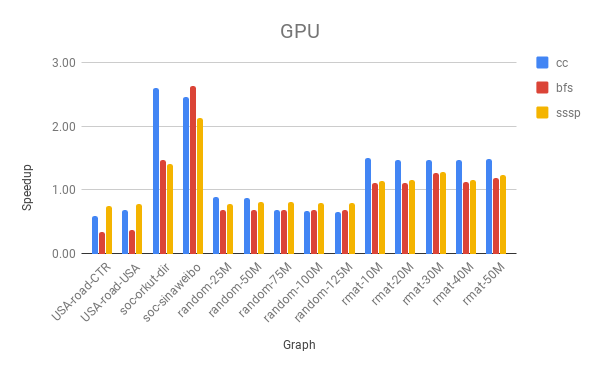
\includegraphics[width=0.7\linewidth]{GPU.png}
\caption{Speedup of edge-based with respect to vertex-based processing in GPU.}
\label{speedup:gpu}
\end{figure}
\begin{figure}
\centering
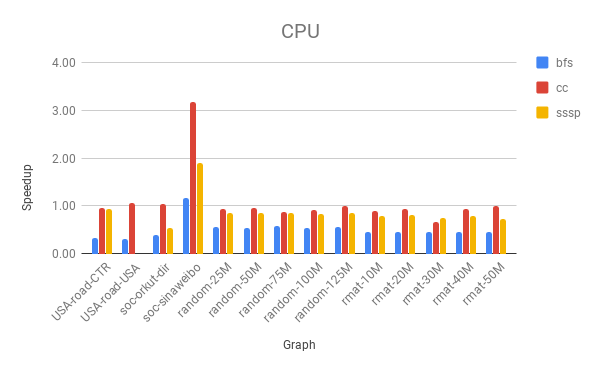
\includegraphics[width=0.7\linewidth]{CPU.png}
\caption{Speedup of edge-based with respect to vertex-based processing in CPU.}
\label{speedup:cpu}
\end{figure}

As we can see from Figure \ref{speedup:gpu}, edge-based processing is performing better in social-network and rmat graphs. It is because degree of vetices in those graph has very high variance and due to this there is thread divergence in GPU, which basically means those threads which are mapped to vertices with less degree will have to wait for the threads which are mapped to high degree vertices for their processing to complete. In edge-based, threads does not have to wait as each of the thread has to process only two vertices which are the source and destination vertex of the edge mapped to the thread. However, we do not see this performance gain in CPU, as we can see from Figure \ref{speedup:cpu}. This is because CPU does not have enough resource to utilize the enough parallelism provided by edge-based processing.

\subsection{Effect of Synchronous versus Asynchronous}\label{expt:syncasync}
\begin{table}
\centering
\begin{tabular}{|l|r|r|}
\hline
\textbf{Graph} & \textbf{Asynchronous}  & \textbf{Synchronous}\\\hline
USA-road-CTR &   106 &   134\\\hline
USA-road-USA &   86 &   91\\\hline
soc-orkut-dir &   285 &   425\\\hline
soc-sinaweibo &   4508 &  8310\\\hline
random-25M &   347 &   458\\\hline
random-50M &   741 &   945\\\hline
rmat-10M &   320 &   329\\\hline
rmat-20M &   665 &   771\\\hline
\end{tabular}
\caption{Execution time (in ms) of benchmark for different graphs in CPU.}
\label{tab:async-cpu}
\end{table}
We can see from Table \ref{tab:async-cpu} that asynchronous version is performing better than synchronous version in case CPU. This is because threads does not have to wait for other threads in case of asynchronous execution. However we don't see performance gain in GPU. The main reason for this is that the graph we took is very large, so there is no resource left in GPU to launch (asynchronously) a different kernel. As a result both the kernels have to execute synchronously.

\subsection{Effect of CPU, GPU \& Multi-GPU Code}\label{expt:cpugpu}
\begin{table}
\centering
\begin{tabular}{|l|r|r|r|}
\hline
\textbf{Graphs} & \textbf{Multi-GPU} & \textbf{GPU} & \textbf{CPU (16 threads)}\\\hline
random-25M \& random-50M & 826  & 1234 & 3866 \\\hline
rmat-10M \& rmat-20M & 792 &  1176 & 3024\\\hline
\end{tabular}
\caption{Execution time (in ms) of \textit{connnected components} for two different graphs.}
\label{tab:multigpu}
\end{table}
To see the effect of CPU, GPU and Multi-GPU code, we have executed connected components algorithm to two different graphs in different backends. Multi-GPU took much less time as compared to other backends, as can be seen in Table \ref{tab:multigpu}. In Multi-GPU, all the graph runs asynchronously in different GPU so the time taken is the max of the two graphs. While in CPU and GPU, both the graphs has to run synchronously. As GPU can utilize more parallelism provided by the algorithm than CPU, so GPU performs better than CPU.

\subsection{Effect of Optimizations}\label{expt:optimizations}
We experimented by running Breadth-first Algorithm, which computes the distance of each vertex from a source vertex, in GPU and finding the distant vertex from source in CPU. It is observed that with optimization program takes less than a second to finish while without optimization program gets timed out (where 5 minute was kept as limit). This is because, without optimization cpu copies distance of each of the node one by one whereas with optimization cpu copies all the distance at once and then uses it for finding maximum distance. As the communication overhead is very high between cpu and gpu, so without optimization is affected badly.

\section{Related Work}\label{sec:related}
Green-Marl~\cite{Hong:2012:GDE:2150976.2151013} is a graph DSL for 
implementing parallel graph algorithms on multi-core CPUs using \texttt{OpenMP}.
 %Green-Marl has separate  data types  {\tt DGraph} and   {\tt UGraph}  for directed and undirected graphs respectively. 
It has two data types {\tt Node} and {\tt Edge} to represent vertices and edges in the graph respectively.
\REM{
 Green-Marl has three types of worklists data types namely {\tt Set}, {\tt Order} and {\tt Sequence}. These data types may contain a set of vertices in a graph. Elements in a {\tt Set} are unique but not ordered. Elements in an {\tt Order} are unique and ordered. Elements in a  {\tt Sequence} are ordered but not unique. 
Green-Marl uses {\tt Foreach} construct for parallelism.

 An example of a {\tt Foreach} statement is given below.\\

{\tt Foreach} (v : G.Nodes) (cond) \{ ... \}\\
Here all the vertices {\it v}  in the graph {\it G}  which satisfy the condition {\it cond} execute the body of the {\tt ForEach} statement. 
There are iterators for vertices ({\tt Node}) in graph like {\tt nbrs} in Green-Marl.}
 Green-Marl does not support mutation of the graph object
(i.e., adding and removing vertices and edges to/from the graph object). So dynamic graph algorithms cannot be written in Green-Marl.
LightHouse~\cite{lighthouse} added CUDA backend to Green-Marl.
\REM{ Green-Marl supports only multi-core CPUs, and  graph algorithms targeting  \GPU devices cannot be programmed in Green-Marl.}
Galois~\cite{Pingali:2011:TPA:1993316.1993501} is a C++ framework for implementing graph algorithms on multi-core CPUs. It supports mutation of graph objects via {\it cautious} speculative execution. 
It uses a {\it worklist} based execution model, where all the {\it active elements} are pushed to a {\it worklist} and are processed in {\it ordered} or {\it unordered} fashion.
\REM{Galois has a {\tt foreach} operator to process active elements in parallel. 
The {\tt foreach} operator takes as argument an  {\it ordered} or {\it unordered} worklist.
 During the processing of {\it active elements}, new {\it active elements} are created, which will be processed in the following rounds of computation. }
Elixir~\cite{Prountzos:2012:ESS:2398857.2384644} is  a graph DSL to  develop and implement parallel graph algorithms for analyzing static (i.e., non-mutable) graphs and it targets multi-core CPUs.
\REM{ Elixir uses both declarative and imperative  constructs for determining computations over a graph. }

X-Stream~\cite{Roy:2013:XEG:2517349.2522740}  uses edge-centric processing for graph applications.
\REM{ rather than using vertex centric processing for algorithms such as SSSP and Strongly Connected Component (SCC)}. 
It supports both in-memory and out-of-core graph processing on a single shared-memory machine using scatter-gather execution model.
The Stanford Network Analysis Platform (SNAP)~\cite{Leskovec:2016:SGN:2973184.2898361} provides high-level operations for large network analysis including social networks and target
multi-core CPUs. 
Ligra~\cite{Shun:2013:LLG:2517327.2442530} is a framework for writing graph traversal algorithms
for multi-core shared memory systems. For vertex- versus edge-based processing, it uses two different routines: one for  mapping  vertices and the other for mapping  edges. However, the DSL code needs modification if one needs to alter the mapping.
Polymer~\cite{Zhang:2015:NGA:2858788.2688507} is a NUMA aware graph framework for multi-core CPUs and it is built
with a hierarchical barrier to get more parallelism and locality. 
The GraphChi~\cite{Kyrola:2012:GLG:2387880.2387884} framework processes large graphs using a
single machine, with the graph being split into  parts, called shards, and loading shards one by one into RAM and then processing each shard. 
Such a framework is useful in the absence of distributed clusters.


\section{Conclusion}\label{sec:conclusion}
Irregular codes have data-dependent access patterns.
Therefore, compilers need to make pessimistic assumptions leading to very conservative code.
While DSLs for irregular codes allow us the flexibility to make more informed decisions about the domain, existing DSLs lack adaptability.
Different graphs expect different kinds of processing to achieve the best performance.
While existing DSLs do allow changing the algorithm specification to be changed to suit a purpose, it would be ideal if the specification remains intact and the compiler judiciously generates the necessary efficient code.
We presented our experiences in achieving the same, for a graph DSL, Falcon.
In particular, we auto-generated codes for vertex-based and edge-based processing, for synchronous versus asynchronous processing, and for CPU versus GPU versus multi-GPU processing.
We illustrated the effectiveness of our techniques using a variety of algorithms and several real-world graphs.
We believe other DSLs would also benefit from our proposal.


\bibliography{refs}
\bibliographystyle{plain}
\end{document}



